\documentclass[a4paper,twoside]{article}

\usepackage{epsfig}
\usepackage{subfigure}
\usepackage{calc}
\usepackage{amssymb}
\usepackage{amstext}
\usepackage{amsmath}
\usepackage{amsthm}
\usepackage{multicol}
\usepackage{eurosym}
\usepackage{apalike}
\usepackage{epstopdf}
\usepackage{float}
\usepackage{SCITEPRESS}     % Please add other packages that you may need BEFORE the SCITEPRESS.sty package.
\usepackage[utf8]{inputenc} %Codificacion utf-8

\setlength\parindent{0pt}
\subfigtopskip=0pt
\subfigcapskip=0pt
\subfigbottomskip=0pt

\begin{document}

\title{Adaptative and personalized web framework for searching data using flexible queries  \subtitle{} }

\author{\authorname{Victor Pablos Ceruelo\sup{1}, Dan Seeruttun - - Marie\sup{1} and Susana Muñoz Hernandez\sup{2}}
\affiliation{\sup{1}PHD in ...,  Universidad Politecnica de Madrid, My Street, MyTown, MyCountry}
\affiliation{\sup{2}Student in Software Engineering, Universidad Politecnica de Madrid, Rennes, France}
\affiliation{\sup{3}Computer Science...,  Universidad Politecnica de Madrid, MySecondTown, MyCountry}
\email{\{victorpablosceruelos, dan.seeruttun\}@gmail.com, susana@fi.upm.es}
}

\keywords{Active learning, Fuzzy logic, Database}

\abstract{The abstract should summarize the contents of the paper and should contain at least 70 and at most 200 words. The text must be set to 9-point font size.}

\onecolumn \maketitle \normalsize \vfill

\section{\uppercase{Introduction}}
\label{sec:introduction}

When trying to model a problem, assigning each concept to a term and an universal meaning is very important. These names must be very clear for anyone. However, problems can appear during the modelization of a fuzzy or subjective problem, where terms meaning vary and are not clear. 

For instance, trying to model the concept of the predicate expensive car is difficult because it involves each person own idea of expensive to represent it.  Secondly, how can a car be defined with an expensive and non expensive term ? If sticking to the reality is an objective, being able to define the expensiveness of any product is the key.

Thus a better representation of the predicate is needed, associating a cost and its match with the predicate is the idea. That's introducing the concept of truth value, seen in (Citation Victor Thesis), a value that will represent the match between fuzzy values and their predicates, or in our example costs and the predicate expensive. With this modelization, it will become possible to search through databases, coupling truth values and fuzzy predicates and even going further by personalizing predicate to users.
In this paper, FLESE will be presented, an implementation of the fuzzy concept through databases, adaptative and able to personalize to each user.

%\section{\uppercase{\uppercase{RFuzzy}}}

\section{\uppercase{\uppercase{Flese}}}

\subsection{\uppercase{Generalities}}

FLESE is an user friendly interface for the search engine provided by Rfuzzy, with the capability to evaluate the (possibly) fuzzy query against a database containing no fuzzy information.\\

By using it we can answer queries like “I want a restaurant close to the center serving Mediterranean food or similar” from a database that contains a list of restaurants with the distance of each one (100 meters, 1000 meters, etc) and the food they serve (Mediterranean, Spanish, Italian, etc) and some meta-information linking fuzzy and non-fuzzy information.

\subsection{\uppercase{Technical overview}}

Flese is composed of an engine, an improved version of RFuzzy: Syntax, semantics and implementation details of a simple and expressive fuzzy tool over Prolog”. In this new framework we have included the management of quantifiers (even negation), similarity, overload of attribute's names and others. \\

Its main advantage over some other engines is that its syntax is trivial, it can use both fuzzy and crisp data, it allows to reuse existing databases and Prolog code and it has every facility we need to represent real-world applications. Rfuzzy is a package of the Ciao Prolog logic programming environment.  \\

The web interface is a Java application that interprets the answers provided by the fuzzy framework. It runs on a Tomcat server behind an Apache proxy.  \\

FleSe core is developed as a Ciao Prolog package, while the web interface is managed by a Java application running on an Apache Tomcat Debian (Linux) server. The client part of the web interface is developed in HTML and JavaScript and uses Ajax to improve the usability. Besides, we use some libraries developed by others. Mainly: SocialAuth, OpenId4Java, jQuery, jQuery UI and Highcharts JS.\\

The architecture is the following figure \ref{fig:architecture}:

\begin{figure}[!h]
  %\vspace{-0.2cm}
  \centering
   {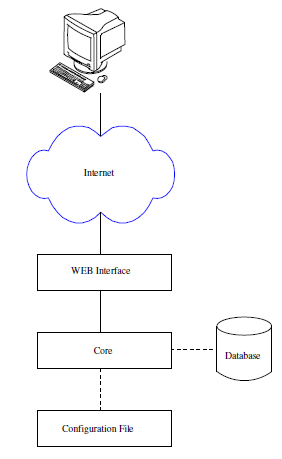
\epsfig{file = archi.png, width = 5.5cm}}
  \caption{FLESE architecture}
  \label{fig:architecture}
 \end{figure}

The users connects himself to Flese's interface. with an Internet Browser. \\
 FleSe’s web interface is an application written Java that runs on a Tomcat server, on a machine with a Linux operating system. The Tomcat server listens to http(s) requests and, when it receives one for the FLESE application, it redirects it to the Servlet in the FLESE application in charge of processing and answering it. \\

In order to process and answer the request the Servlet evaluates what it is asking for and decides whether it needs to call the core for answering it or not. When we press the search button most of the times it calls the core, but if the query has been posed recently it will use cached results to decrease the response time. \\

The core is RFuzzy, a Prolog program that reads a prolog configuration file to determine to which database connect to (and how),  link multiple tables into a virtual database table or get rid of columns with not needed information, give meaning to each column in the virtual database table and add concepts (fuzzy or not) to the list of concepts with which the user can build queries. Once the configuration file is chosen by the user the web interface asks the core to load it. \\

To increase the speed of answering a query, the most common queries are pre-cached. In others words, the most repetitive data and its similar queries are kept in the cache.

\subsection{\uppercase{Fuzzy processing}}

The system has got semantic recognition, it can recognize the queries it can process and orient the user with its interface, or it can refuse if it is not possible.\\
For this semantic recognition, the file owner has to implement what are the words used in queries, defining them with direct access to the database or combining data from it:


\begin{small}
\begin{verbatim}
     near_the_city_center(restaurant):~ 
function(distance_to_the_city_center(restaurant),
 [ (0, 1), (100, 1), (1000, 0.1) ]).
\end{verbatim}
\end{small}

Combining easily predicates make the file owner free to implement whatever he wants. He can as well implement similarities between predicates. If the user wants to access a Mediterranean restaurant, there is no easy decomposition of this definition, but it can be defined combining other predicates with similarities. \\
The data is computed by the core, and the solutions of the query are displayed on Flese, ordered by their truth value, a value between 0 and 1 that determines the validity of the solution.

\begin{small}
\begin{verbatim}
    define_similarity_between
(restaurant, food_type(mediterranean), 
food_type(spanish), 0.8) cred (prod, 0.9).
\end{verbatim}
\end{small}

\subsection{\uppercase{Flese Interface}}
Each user has to identify himself to Flese via a Social network provider, and then he gets access to the application. The user can add his configuration file, or browse the one already existing.\\

One of the advantages of Flese is it can work with more than one database for the queries, and you can have access not only to your file, but to the files other users shared.\\

To make a query, first the user has to choose the subject of his query, and then the predicates available are displaying, fuzzy and crisp, using the core of Rfuzzy. Some of the queries have more data to insert than others, it will be displayed automatically, like in Figure \ref{fig:predicate}.\\

\begin{figure}[!h]
  %\vspace{-0.2cm}
  \centering
   {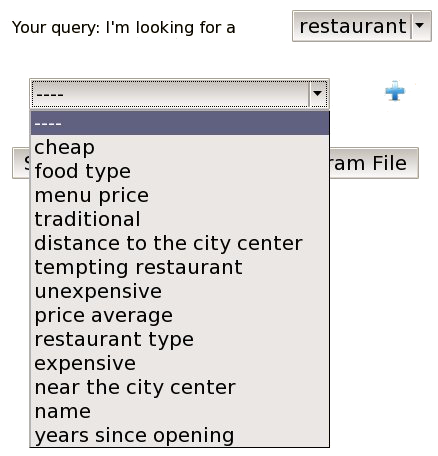
\epsfig{file = predicate.png, width = 5.5cm}}
  \caption{List of predicates}
  \label{fig:predicate}
 \end{figure}

Modifiers are as well available, like negation \textit{Not}, minimum \textit{Min}, and quantity modifiers are accessible too like \textit{very}, or \textit{too much}. For the numerics predicates, it is possible to use comparisons operators to complete more complex queries, like in figure \ref{fig:min}, \ref{fig:op}, and \ref{fig:query}.\\

\begin{figure}[H]
  %\vspace{-0.2cm}
  \centering
   {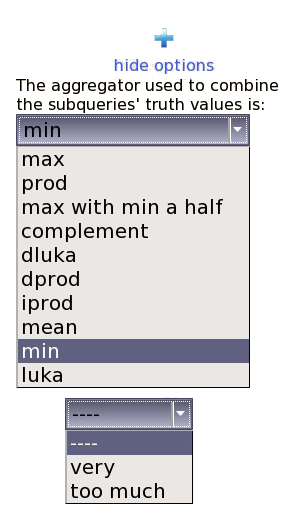
\epsfig{file = min.png, width = 5.5cm}}
  \caption{Available functions}
  \label{fig:min}
 \end{figure}

\begin{figure}[H]
  %\vspace{-0.2cm}
  \centering
   {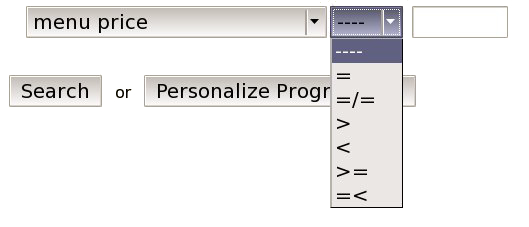
\epsfig{file = op.png, width = 5.5cm}}
  \caption{Available operators }
  \label{fig:op}
 \end{figure}

\begin{figure}[H]
  %\vspace{-0.2cm}
  \centering
   {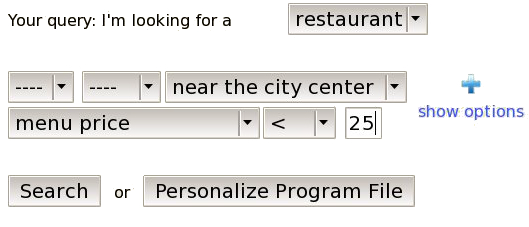
\epsfig{file = query.png, width = 5.5cm}}
  \caption{Example of query}
  \label{fig:query}
 \end{figure}


Finally, the results is displayed on a table, provided and ordered with the truth value in the figure \ref{fig:results}.

\begin{figure}[H]
  %\vspace{-0.2cm}
  \centering
   {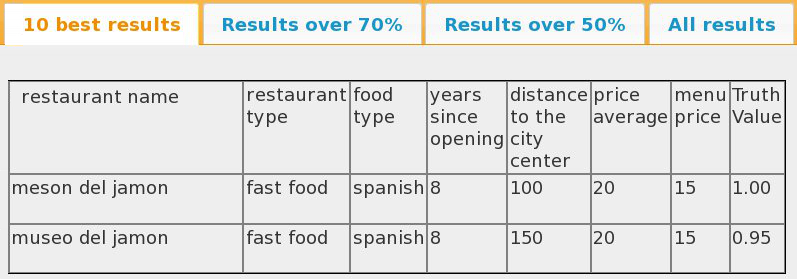
\epsfig{file = results.png, width = 8 cm}}
  \caption{Example of results}
  \label{fig:results}
 \end{figure}

\newpage


\section{\uppercase{\uppercase{Adaptative personalized framework}}}

\subsection{\uppercase{user personalization}}

Flese application brings the treatment of the fuzzy queries but it does not solve the problem of the subjectiveness of the fuzzy queries. Indeed, an expensive car does not have the same meaning for everyone.\\

The point of the user personalization is to give to the user the opportunity to modify the definition of the fuzzy predicates, thus to overcome the subjectivity of the vocabulary used. Moreover, a personalization does not affect other users, so each user can create his own definitions of the same predicate to access the same database using Flese. The database file will then contain all users personalization.\\

To personalize a predicate, the predicate is divided in sections that can be personalized by the user. Consequently, not all the predicate can be personalized. For example, let the predicate "height of car in mm". This predicate is non fuzzy and it is impossible to personalize it. Furthermore, the owner of the file can decide or not to let users personalize a predicate. \\

To make a predicate personalizable, the owner of the file has to divide the predicate in sections. The user will be able to assign values to each sections. For instance, using the predicate expensive, these could be the different sections to take into account.

\begin{itemize}
    \item From 0 \euro\ to 10000 \euro
    \item  From 10000 \euro\ to 30000 \euro
    \item  From 30000 \euro\ to 100000 \euro
    \item  More than 100000 \euro
\end{itemize}

At each section will be associated a truth value, and this value is the one the user will be able to edit.\\

This algorithm is the first default function for the predicate price\_in\_euros applied to car. The first value is the price and the second is the truth value. \\

\subsection{\uppercase{Implementation on Flese}}

The system of sections has been implemented on Flese. 
To authorize the modification of the file, the prolog syntax of the file for the predicate expensive is the following:

\begin{small}
\begin{verbatim}
     expensive(car) :~
 function(price_in_euros(car), [ (0, 0),
 (10000, 0.5), (30000, 1), (100000, 1) ]).
\end{verbatim}
\end{small}

Let's demonstrate the usefulness of this fuzzy predicate personalization. \\
 We choose a user that is looking for an expensive car. If he runs the query directly, he will find the following solutions in the table \ref{tab:simpleQuery1}: \\

\begin{table}[h]
\caption{Results of simple expensive car query}\label{tab:simpleQuery1} \centering
\begin{tabular}{|c|c|c|c|}
  \hline
  N0 & Name & Price & Truth value\\
  \hline
  1 & VW Caddy & 45000 & 1\\
  \hline
  2 & Alfa Romeo & 30000 & 1 \\
  \hline
  3 & Aston Martin & 150000 & 1 \\
  \hline
  4 & Ford S Maxi & 30000 & 1 \\
  \hline
  5 & Audi TT & 40000 & 1 \\
  \hline
  6 & Audi Quattro & 48000 & 1 \\ 
  \hline
\end{tabular}
\end{table}

The 6 first results will be expensive car with a truth value of 1, this table of results will not please a rich user, that will be interested in a higher cost for the predicate expensive. \\

Then he will assign a truth value to different ranges of prices, from inferior to 10000 \euro\\  to more than 100000 \euro . A rich user may personalize this predicate imposing that a car valued at 30000 \euro\  is not really expensive (truth value = 0.40) and a car valued at 100000 \euro\  is very expensive (truth value = 1). After being modified, a message appears confirming the modification. The figure \ref{fig:fuzzypers} illustrates this example. \\

\begin{figure}[!h]
  %\vspace{-0.2cm}
  \centering
   {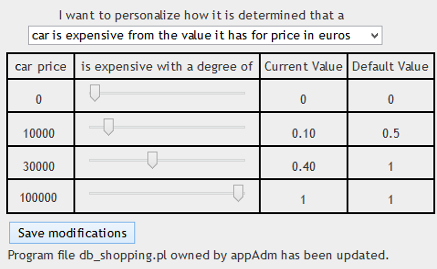
\epsfig{file = pers.png, width = 8cm}}
  \caption{Fuzzification personalization.}
  \label{fig:fuzzypers}
 \end{figure}

After having modified the predicate, the user can still have a look to the default value of the predicate in case of he is lost. This part remains important to help the user to get back from a wrong personalization. The result of the query is presented in the table \ref{tab:solveQuery1}:  \\ 

\begin{table}[h]
\caption{Results of fuzzy expensive car query}\label{tab:solveQuery1} \centering
\begin{tabular}{|c|c|c|c|}
  \hline
  N0 & Name & Price & Truth value\\
  \hline
  1 & Aston Martin & 150000 & 1 \\
  \hline
  2 & VW Caddy & 45000 & 0.55\\
  \hline
  3 & Audi TT & 40000 & 0.49 \\
  \hline
  4 & Audi Quattro & 48000 & 0.41 \\ 
  \hline
  5 & Alfa Romeo & 30000 & 0.4 \\
  \hline
  6 & Ford S Maxi & 30000 & 0.4 \\
  \hline
\end{tabular}
\end{table}
% 70000*0.4/0.6-16667


Asking for his expensive car, the user knows by reading the truth values that there is only one expensive car according to his definition. The user is taking into account only the cars with truth values around 1. The advantage of the truth values is the user can easily select the expensive cars with a 60% conformance with the definition just by watching the truth values. In that case, only the Aston Martin car will appears in the ranking. \\

The owner of the file can decide which predicate he wants to authorize the personalization. He keeps the control on the file, he can impose a default value of the fuzzification before any personalization. \\

\subsection{\uppercase{Machine learning for improving searching criteria}}

Starting considering an increasing number of users, it becomes interesting to search for better predicate criteria. Indeed, the users joining the application after the others can benefit from the others data. Knowing that people share some predicate personalization can lead to an improvement of the criteria for the newcomers. In that sense, Flese changes the values of the default function for the newcomers' and non personalized's predicate according to what is most representative to the users. \\

The owner of the file has access to all predicate personalisation and can see their representation to understand better the sample of population. Knowing that the predicate are divided in sections that are independant from each others, the algorithm is applied on each of these sections individually. \\

The median has been chosen for this algorithm to fit with the higher number of people's criteria, so the new user won't have to personalize the fuzzification, or only parts of it. Moreover, the median is better than a simple average because the value will fit an actual personalization. It become important on the case we have 2 opposites types of population. The average algorithm will give us an average value, that will fit none of the 2 types of the population.\\

Meanwhile the median algorithm will give us the personalization of one user belonging to the biggest population. That is why the median algorithm is better.\\

Theses changes will have no effect on the parametrized fuzzification if it has been already changed. For example, given a population A and a population B having different behaviours with the predicate expensive, if we introduce more people of population A than people of population B, the definition of the predicate will adapt to the situation, following the population A predicates. \\

The searching criteria will then adapt to the population of the users. Even after deciding to invert the population rate, by adding more poor people, the predicate criteria will be personalized by the new population to fit their idea. In that case, the criteria will represent more the poor people. \\

For instance, if most of the people consider that 10000 \euro\  and 30000 \euro\  is not expensive, the default expensive predicate will adapt according to it. Here is an example showing the adaptation in figure \ref{fig:activelearning}:


\begin{figure}[H]
  %\vspace{-0.2cm}
  \centering
   {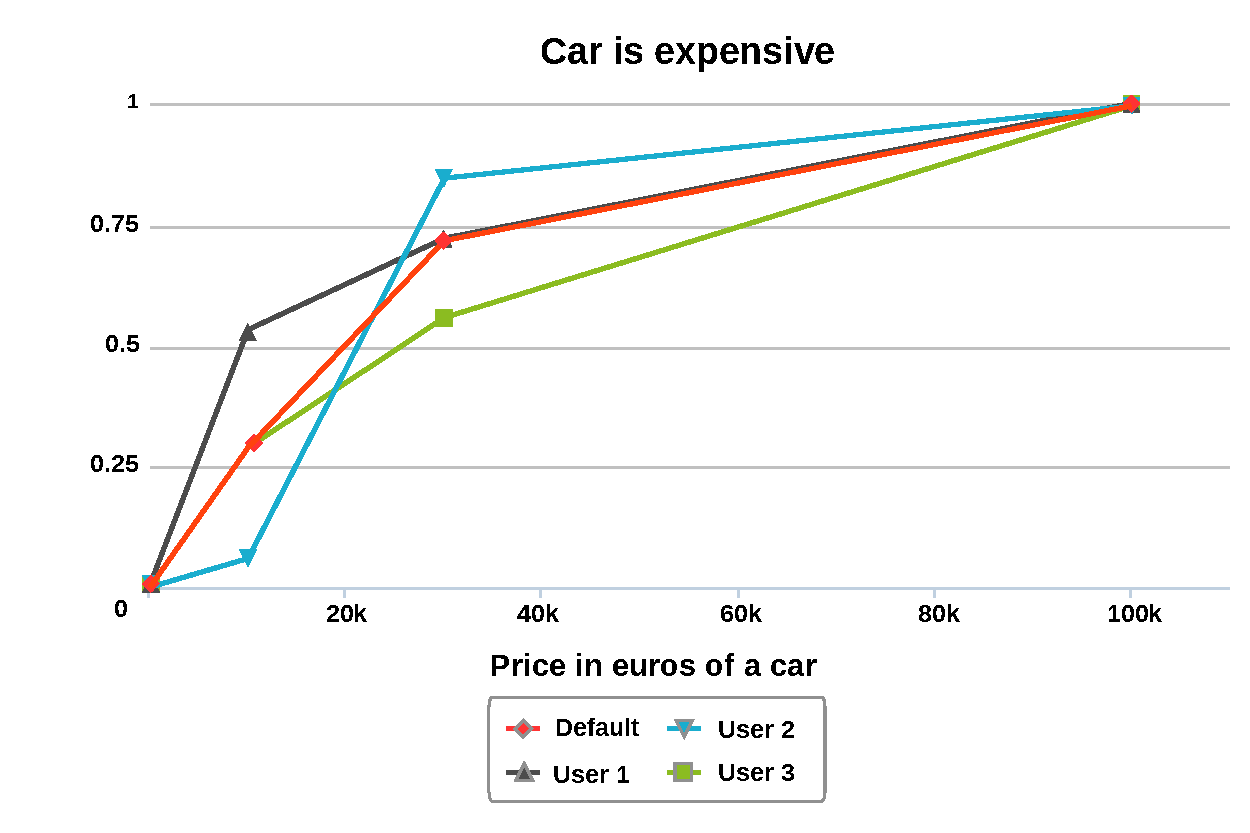
\epsfig{file = chart.pdf, width = 8 cm}}
  \caption{Default function determined by active learning.}
  \label{fig:activelearning}
 \end{figure}

In this example, 3 users personalized the predicate expensive. The Default function follows the median algorithm for each section. \\

For 10000 \euro\, it is following the user3, and for 30000 \euro\, it is following the user 1. The point of this figure is to show that the Default function is able to fit with most of the population of users.

\newpage

\section{\uppercase{Conclusions}}
\label{sec:conclusion}

Today, to represent the real world, we need to handle fuzzy data. Thanks to Flese, it is possible to launch fuzzy queries on a crisp prolog database. \\

The objectif is to get closer to the real language, to improve the semantic of the query. It is involving comparators, quantifiers, operators to create the maximum of queries. Consequently, even users with few computer science knowledge can run a query through the application. \\

Every user has different notions of fuzzy predicates. The better way to handle it is not to impose them our way, but to grant them the right to edit it. With the median algorithm, it is possible to assign a good value to the default predicate, and this default predicate will fit better with the user's population. Flese is adaptable and personalizable for each users.



\vfill
\bibliographystyle{apalike}
{\small
\bibliography{example}}


\section*{\uppercase{Appendix}}

If any, the appendix should appear directly after the
references without numbering, and not on a new page. To do so please use the following command:
\textit{$\backslash$section*\{APPENDIX\}}

\vfill
\end{document}

